%% ----------------------------------------------------------------
%% AppendixA.tex
%% ---------------------------------------------------------------- 


\chapter{Appendix} \label{Chapter:Appendix}

The StackOverflow website had be analyzed to see the formation of purposive social network and users communication network is studied. Chapter 4 includes many of the important graph, charts and histograms showing user interactions and activities. Some more of user activity has been analyzed but it was not included in the chapter. Some of the charts are as follows:

\section{User activity}

StackOverflow is a USA based website and since it is an english language website, many of the users are from english speaking nations and from western countries. Analysis of users activities by hour shows when user interact the most. 

\begin{figure}[!htb]
  \centering
  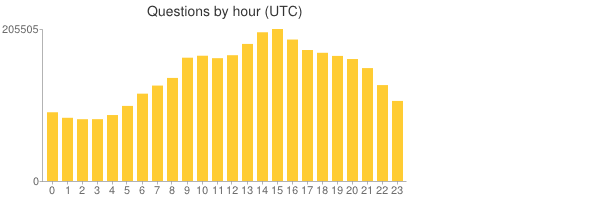
\includegraphics[width=15cm]{chart8.png}
  \caption{Questions posted by the hour}
  \label{Figure:figexa1}
\end{figure}

\begin{figure}[!htb]
  \centering
  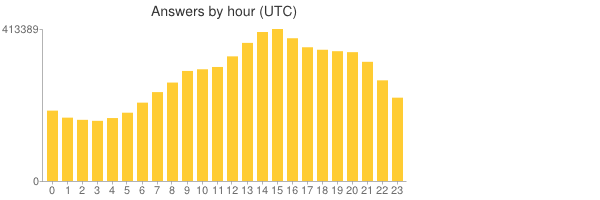
\includegraphics[width=15cm]{chart9.png}
  \caption{Answers posted by the hour}
  \label{Figure:figexa2}
\end{figure}

As can be seen from the figures above, afternoon is the most active time for the users to post questions and answers in the USA time zone. Also, 9 and 10 am in the morning, the afternoon time for some part of Asia and Europe also shows some rise in user activity. Geographical analysis of the website suggests that most of the registered users are from USA and then from Europe.